\section{Simulation Results}
The numerical experiment in this section simulates one leader-follower tractor pair. Figure \ref{fig:Leader_Follower_Simulation_Results_2DPlot} shows the path traversed of both tractors along with snapshots of position for initial and terminal simulation positions. Way points that are lateral offsets of the leader's trajectory used for follower heading correction are denoted as circles and the x denotes the current way point being used. Figure \ref{fig:Leader_Follower_Simulation_Results_Traj} shows plots of vehicle speed $v_T$, yaw rate $\dot\theta$, left and right slip ratios $i_L$ and $i_R$, engine speed $\Omega_E$ and drawbar arm angle $\phi$. Initial $[X,Y]$ starting locations for the leader and follower are $[120, 210]$ and $[70, 209]$ respectively. This corresponds to a column formation where the follower vehicle lateral offset is $D_{lat}= 1m$ and the longitudinal offset is $D_{long} = 40m$. The manned leader's trajectory is dictated using a combination of open loop and closed-loop commands. Open loop commands include throttle , $\Pi_{leader} = [0.9, 0.9  ,0.9, 0.98]^T$, and gear selections, $g_{GR,leader} = [ 9 , 10 , 11 , 12]^T$, for the time vector $t = [0 , 3 , 8 , 20]^T$ seconds. Closed-loop commands for heading are regulated using a PI contorller and generated using a sequence of two leader way points with $[X_{WP,L},Y_{WP,L}] = [210,1000]$ for $ t \in [0,20)$ seconds and $[X_{WP,L},Y_{WP,L}] = [20,1000]$ for $ t \in [20,60]$ where $X_{WP,L}$ and $Y_{WP,L}$ are the X and Y coordinates the leader drives towards. Controller gains for leader heading correction are $K_{p,\theta} = 2\frac{deg}{deg}$ and $K_{i,\theta} = 0.05\frac{deg}{deg}$. Initially the leader vehicle drives straight but the second way point in the sequence forces it to take an abrupt right turn. This is intentionally induced into the simulation so that payload stability issues are elicited. This is illustrated in the bottom right plot as the drawbar arm angle $\phi$ in Fig. \ref{fig:Leader_Follower_Simulation_Results_Traj} has large oscillations. The advantage of maintaining a flexible formation using the look ahead approach described in Section \ref{s:Way_Point_Following} is that the follower vehicle does not need to mimic the leader's nominal trajectory as with other techniques.Instead, this strategy forces the follower vehicle to make several minor corrections ahead of time to loosely follow the the way point path. The benefit from using this approach can be seen when comparing the trajectory of the drawbar arm angle of the leader and follower in Fig. \ref{fig:Leader_Follower_Simulation_Results_Traj}. The oscillations that are present in the leader's trajectory are rejected by the follower to maintain the payload stable at the rear of the tractor. The controller gains for the follower in this numerical experiment are $k = 0.25\frac{m/s}{m}$, $K_{p,v} = 2 \frac{m/s}{m/s}$, $K_{p,i} = 1\frac{m/s}{m/s}$, $K_{p,\theta} = 2\frac{deg}{deg}$ and $K_{i,\theta} = 0.1\frac{deg}{deg}$. The look ahead distance $D_{LA}$ is set to 40m.

Optimal leader tractor operation occurs when throttle and gear selection inputs are chosen to maximize engine output power and vehicle speed to minimize round-trip traverse times. In theory, the lead vehicle should operate with a throttle command of $\Pi_{leader} = 1$ in the highest gear selection possible. However, in simulations using this open-loop throttle command, the follower tractor has difficulty maintaining the specified formation offset. This is due to the fact that no additional torque is available if the unmanned tractor falls behind due to any disturbance. Furthermore, if the follower tractor has to make heading corrections to follow the way point path, no additional torque is available to power the differential steering hydraulics. Consequently, some limitations on the manned leader's throttle input are required. Simulation results show $\Pi_{leader} \leq 0.98$ to be sufficient. The effect of an additional load from the differential steering hydraulics can be seen when looking at plots of engine speed in Fig. \ref{fig:Leader_Follower_Simulation_Results_Traj} between 30-40 seconds where both vehicles see a reduction in engine RPM.
\begin{figure}[hb]
    \centering
    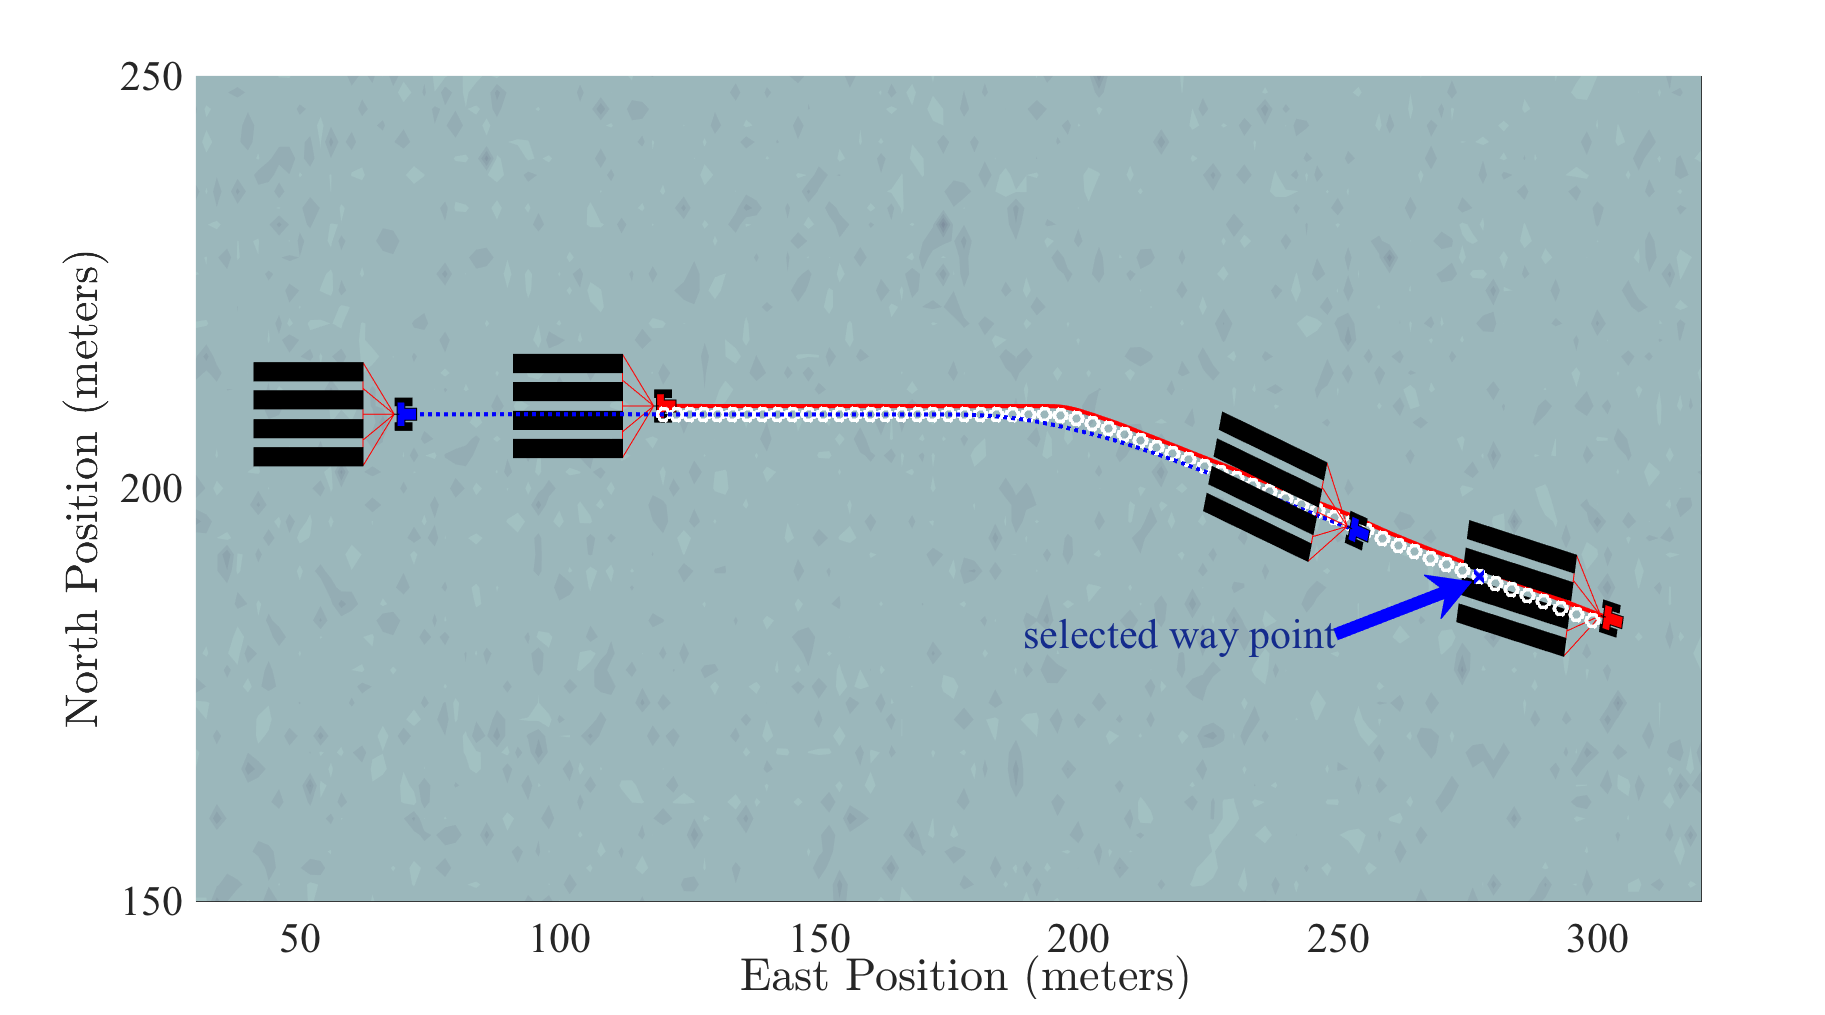
\includegraphics[width=5.5in]{Leader_Follower_Simulation_Results_2DPlot}
    \caption{One leader-follower tractor pair. Starting locations are $[120, 210]$ and $[70, 209]$ for the leader and follower respectively. Snapshots of both vehicles are taken at the starting and terminal locations of the simulation. The paths traversed of each tractor for the leader and follower are highlighted as red, solid and blue, dotted lines. Way points used for follower heading correction are denoted as circles. The way point that is selected at the end of the simulation for heading correction has a x over top of the waypoint circle.}
    \label{fig:Leader_Follower_Simulation_Results_2DPlot}
\end{figure}
\begin{figure}[ht]
    \centering
    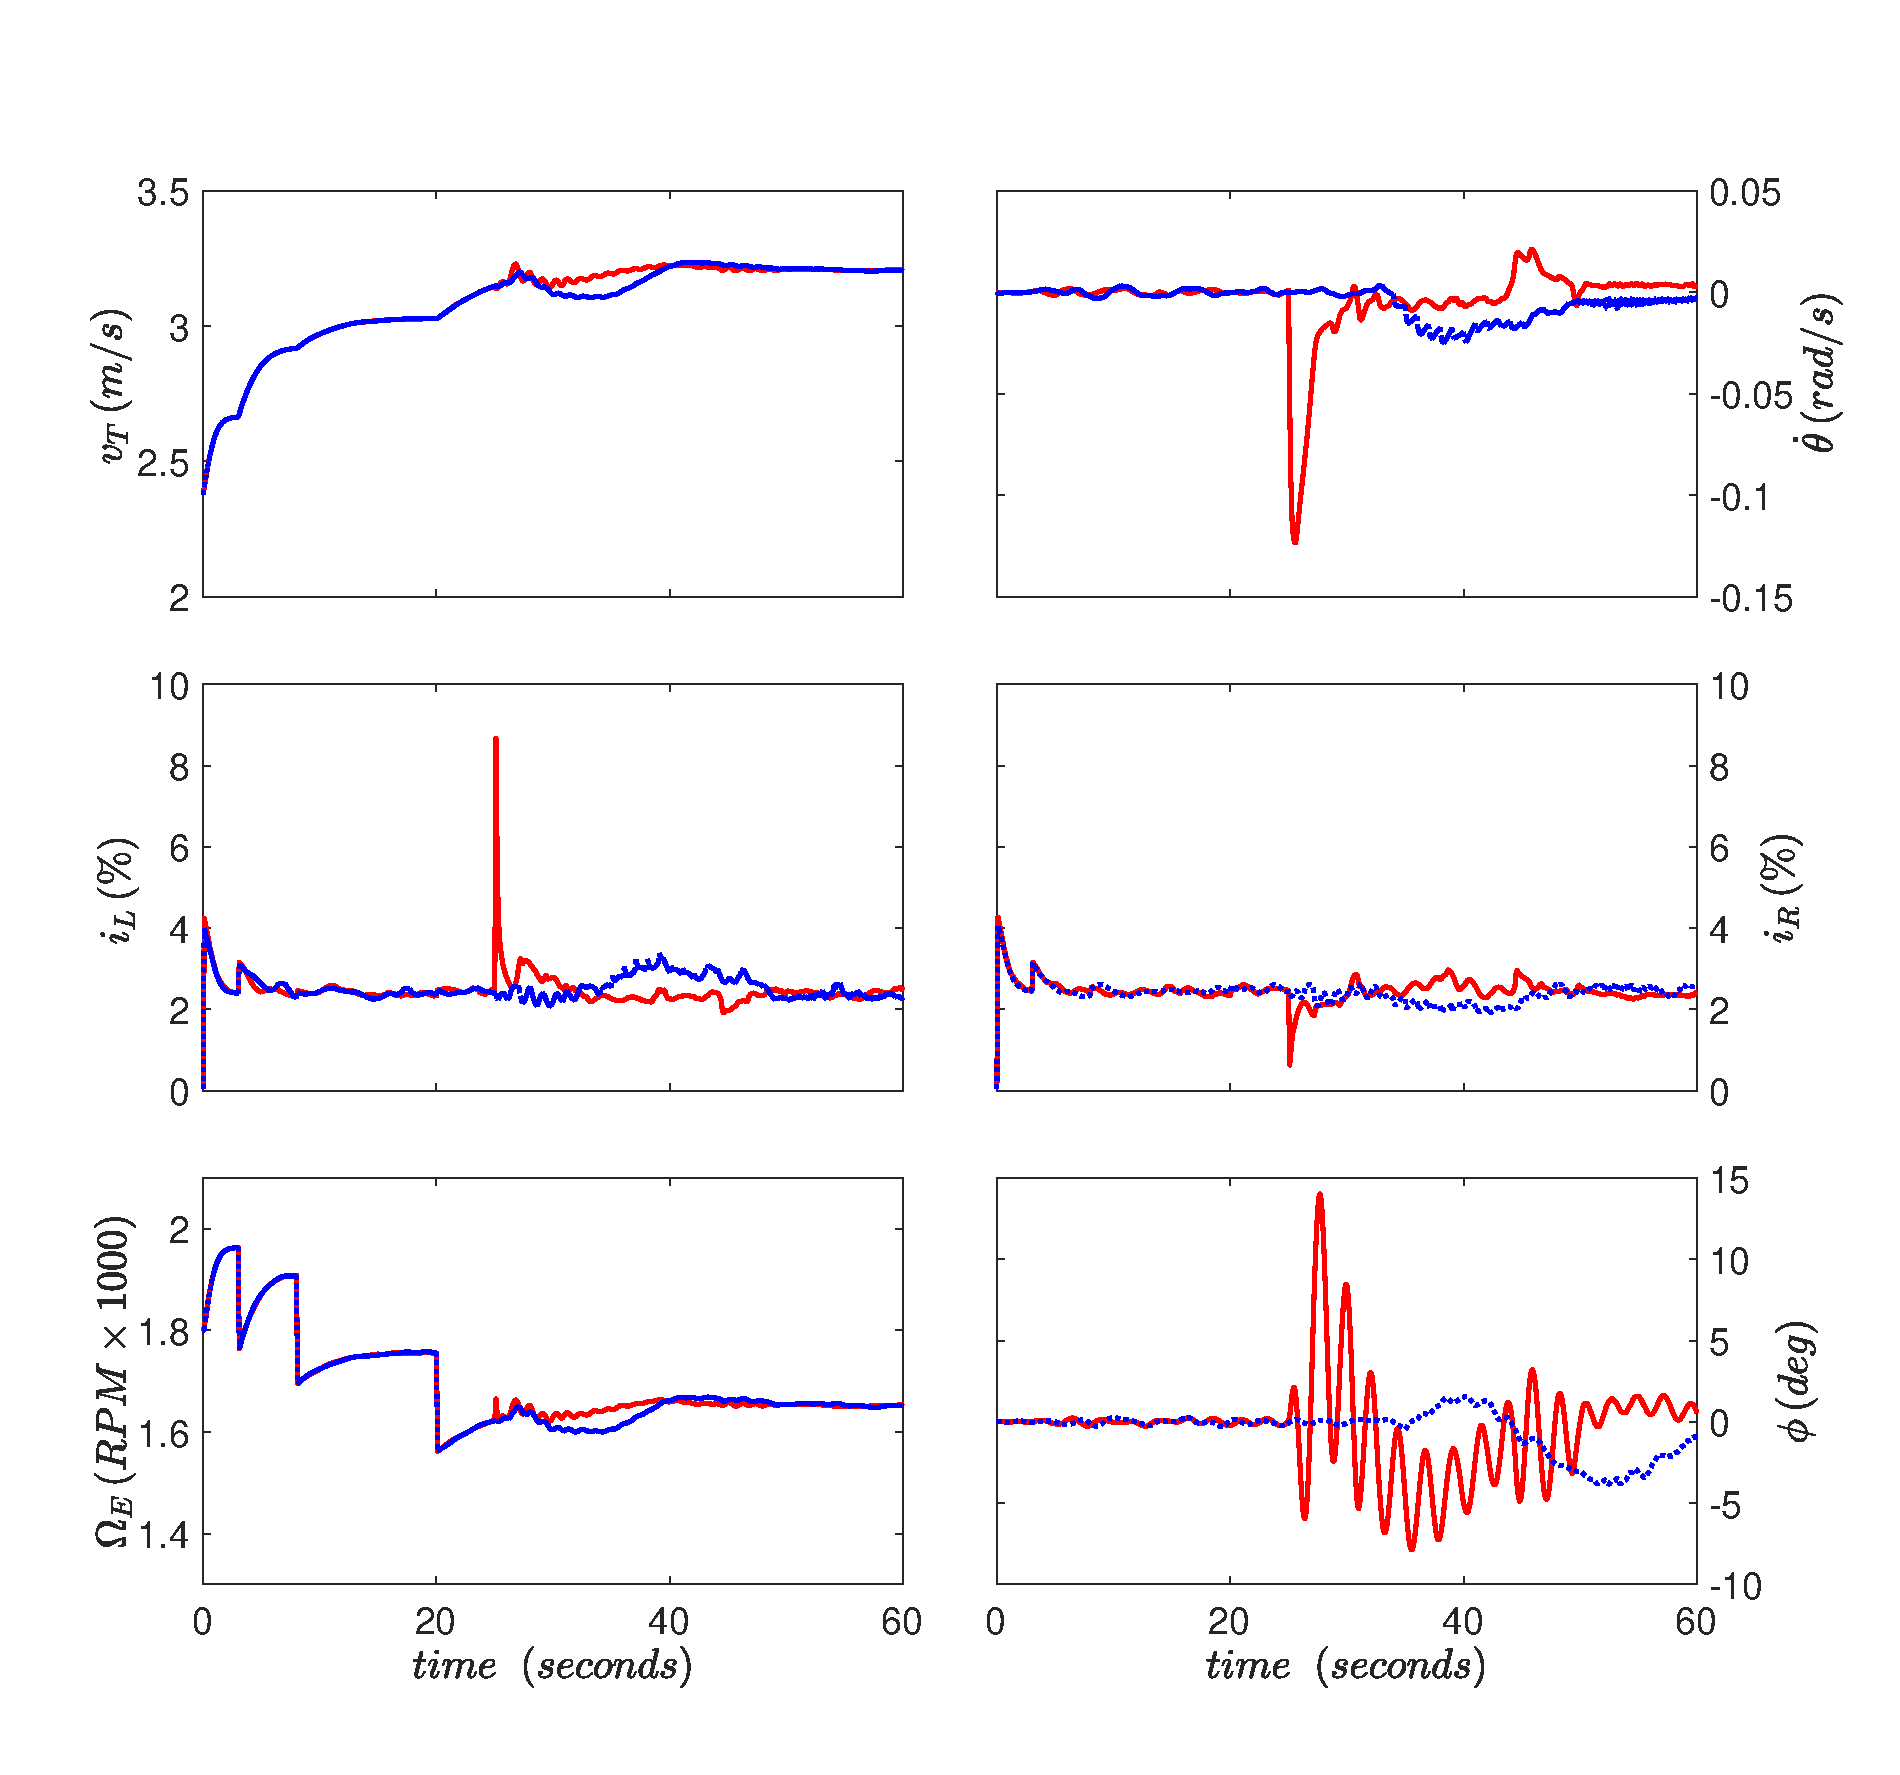
\includegraphics[width=6in]{Leader_Follower_Simulation_Results_Traj}
    \caption{Plots of vehicle speed $v_T$, yaw rate $\dot\theta$, left and right slip ratios $i_L$ and $i_R$, engine speed $\Omega_E$ and drawbar arm angle $\phi$ for the manned leader and unmanned follower tractors. The manned leader's and unmanned follower's trajectories are solid and dotted lines respectively.}
    \label{fig:Leader_Follower_Simulation_Results_Traj}
\end{figure}
